% !TEX root = paper.tex

\section{Algorithm} 
\label{sec:algorithm}

\subsection{Dimension Trees}

An important optimization of the CP-ALS algorithm is to re-use temporary values across inner iterations \cite{PTC13a,KU16-TR,LCPSV17,Kaya17}.
To illustrate the idea, consider a 3-way tensor $\T{X}$ approximated by $\dsquare{\M{U},\M{V},\M{W}}$ and the two MTTKRP computations $\underline{\Mz{X}{1}(\M{W}}\Khat\M{V})$ and $\underline{\Mz{X}{2}(\M{W}}\Khat\M{U})$ used to update factor matrices $\M{U}$ and $\M{V}$, respectively.
The underlined parts of the expressions correspond to the shared dependence of the outputs on the tensor $\T{X}$ and the third factor matrix $\M{W}$.
Indeed, a temporary quantity, which we refer to as a \emph{partial MTTKRP}, can be computed and re-used across the two MTTKRP expressions.
We refer to the computation that combines the temporary quantity with the other factor matrix to complete the MTTKRP computation as a multi-tensor-times-vector or \emph{multi-TTV}, as it consists of multiple operations that multiply a tensor times a set of vectors, each corresponding to a different mode.
This terminology was used in \cite{HBJT17-TR}.

For a larger number of modes, a more general approach can organize the temporary quantities to be used over a maximal number of MTTKRPs.
The general approach can yield significant benefit, decreasing the computation by a factor of approximately $N/2$ for dense $N$-way tensors.
The idea is introduced in \cite{PTC13a}, but we adopt the terminology and notation of \emph{dimension trees} used in \cite{KU16-TR,Kaya17}.
In this notation, the root node is labeled $\{1,\dots,N\}$ and corresponds to the original tensor, a leaf is labeled $\{n\}$ and corresponds to the $n$th MTTKRP result, and an internal node is labeled by a set of modes $\{i,\dots,j\}$ and corresponds to a temporary tensor whose values contribute to the MTTKRP results of modes $i,\dots,j$.

\Cref{fig:DT} illustrates a dimension tree for the case $N=5$.
Various shapes of binary trees are possible \cite{PTC13a,Kaya17}.
For dense tensors, the computational cost is dominated by the root's branches, which correspond to partial MTTKRP computations.
All other edges in a tree correspond to multi-TTVs and are typically much cheaper.

\begin{figure}
% !TEX root = ../paper.tex

\begin{center}
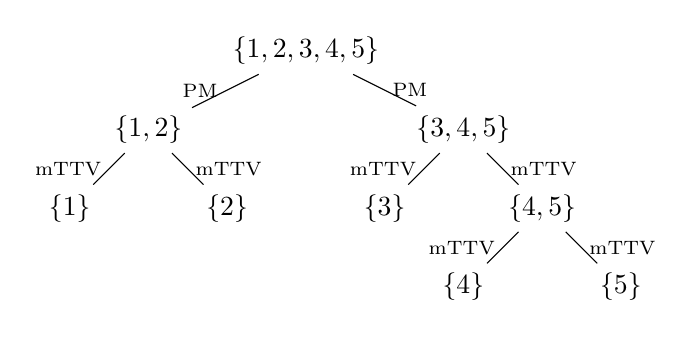
\begin{tikzpicture}

\node (12345) at (4,2) {$\{1,2,3,4,5\}$};
\node (12) at (2,1) {$\{1,2\}$};
\node (345) at (6,1) {$\{3,4,5\}$};
\node (1) at (1,0) {$\{1\}$};
\node (2) at (3,0) {$\{2\}$};
\node (3) at (5,0) {$\{3\}$};
\node (45) at (7,0) {$\{4,5\}$};
\node (4) at (6,-1) {$\{4\}$};
\node (5) at (8,-1) {$\{5\}$};

\scriptsize
\path[draw] (12345) edge [left,align=right] node {PM} (12);
\path[draw] (12345) edge [right,align=left] node {PM} (345);
\path[draw] (12) edge [left,align=right] node {mTTV} (1);
\path[draw] (12) edge [right,align=left] node {mTTV} (2);
\path[draw] (345) edge [left,align=right] node {mTTV} (3);
\path[draw] (345) edge [right,align=left] node {mTTV} (45);
\path[draw] (45) edge [left,align=right] node {mTTV} (4);
\path[draw] (45) edge [right,align=left] node {mTTV} (5);
\normalsize

\end{tikzpicture}
\end{center}
\caption{Dimension tree example for $N=5$. 
The data associated with the root node is the original tensor, the data associated with the leaf nodes are MTTKRP results, and the data associated with internal nodes are temporary tensors.  
Edges labeled with PM correspond to partial MTTKRP computations, and edges labeled with mTTV correspond to multi-TTV computations.}
\label{fig:DT}
\end{figure}

\subsection{Relative Error Computation}

Given a model $\T{M}=\CP$, we compute the relative error $\|\TA - \T{M}\|/\|\TA\|$ efficiently by using the identity $\|\TA-\T{M}\|^2 = \|\TA\|^2 - 2\langle \TA, \T{M} \rangle + \|\T{M}\|^2.$
The quantity $\|\TA\|$ is fixed, and the other two terms can be computed cheaply given the temporary matrices computed during the course of the BCD algorithm.
The second term can be computed using the identity $\langle \TA, \T{M} \rangle = \langle \Mn{M}{N}, \Mn{H}{N} \rangle$, where $\Mn{M}{N} = \Mz{A}{N} (\Mn{H}{N-1} \Khat \cdots \Khat \Mn{H}{1})$ is the MTTKRP result in the $N$th mode.
The third term can be computed using the identity $\|\T{M}\|^2 = \V{1}^\Tra(\Mn{S}{N} \Hada \MnTra{H}{N} \Mn{H}{N})\V{1}$ where $\Mn{S}{N}=\MnTra{H}{1} \Mn{H}{1} \Hada \cdots \Hada \MnTra{H}{N-1} \Mn{H}{N-1}$.
Both matrices $\Mn{M}{N}$ and $\Mn{S}{N}$ are computed during the course of the BCD algorithm for updating the factor matrix $\Mn{H}{N}$.
The extra computation involved in computing the relative error is negligible.
These identities have been used in previous work \cite{KB09,TensorBox,SK16}.

\subsection{Parallel Algorithm}

\subsubsection{Algorithm Overview}

\subsubsection{Data Distribution}

\subsubsection{Inner Iteration}

\subsubsection{Analysis}

\paragraph{Computation}

\paragraph{Communication}

\paragraph{Memory}

% !TEX root = ../paper.tex

\newcommand{\procdim}{3}
\newcommand{\proc}{\draw[black,shift={(-.5,-.5)}] (0,0) grid (\procdim,\procdim);}
\newcommand{\highlight}{gray!75}
\newcommand{\commhighlight}{gray!25}
\newcommand{\parscale}{.46}
\newcommand{\secfaclabel}{$\Mn{M}{2}$}

\newcommand{\parbasepic}{
% highlight one processor's data
% front face
\begin{scope}[canvas is yz plane at x=.5,shift={(1.5,-1.5)}]
	% highlight front face of tensor block
	\draw[fill=\highlight,shift={(0,1)}] (0,0) rectangle (1,1);
	% highlight block of 1st factor matrix
	\draw[fill=\highlight,shift={(-2.5,2-1/3)},xscale=.5] (0,0) rectangle (-1,-1/9);
	% highlight block of 2nd factor matrix
	\draw[shift={(0,-1.5)},yscale=.5] (0,0) rectangle (1/9,-1);
\end{scope}
% right face
\begin{scope}[canvas is zx plane at y=(\procdim-.5),rotate=-90,shift={(-.5,-3)}]
	% highlight front face of tensor block
	\draw[fill=\highlight,shift={(0,2.5)}] (0,0) rectangle (1,1);
	% highlight block of 3rd factor matrix
	\draw[fill=\highlight,yscale=.5] (0,0) rectangle (1/9,-1);
\end{scope}
% top face
\begin{scope}[canvas is yx plane at z=.5,yscale=-1,rotate=0]
	% highlight front face of tensor block
	\draw[fill=\highlight,shift={(1.5,-.5)}] (0,0) rectangle (1,1);
\end{scope}

% draw tensor
% front face
\begin{scope}[canvas is yz plane at x=.5,rotate=-90]
	\proc
\end{scope}
% top face
\begin{scope}[canvas is yx plane at z=.5,yscale=-1,rotate=0]
	\proc
\end{scope}
% right face
\begin{scope}[canvas is zx plane at y=(\procdim-.5),rotate=180]
	\proc
\end{scope}

% draw factor matrices
% front face
\begin{scope}[canvas is yz plane at x=.5,shift={(1.5,-.5)}]
	% draw 1st factor matrix
	\draw[shift={(-2.5,0)},xscale=.5] (0,-2) grid (-1,1);
	\node[draw=none] at (-3.6,-.5) {\Large $\Mn{H}{1}$};
	% draw 2nd factor matrix
	\draw[shift={(0,-2.5)},yscale=.5] (-2,0) grid (1,-1);
	\node[draw=none] at (-.5,-3.5) {\Large \secfaclabel};
\end{scope}
% right face
\begin{scope}[canvas is zx plane at y=(\procdim-.5),rotate=-90,shift={(1.5,-.5)}]
	% draw 2nd factor matrix
	\draw[shift={(0,-2.5)},yscale=.5] (-2,0) grid (1,-1);
	\node[draw=none] at (-.5,-3.5) {\Large $\Mn{H}{3}$};
\end{scope}
}
\begin{figure*}[t]
\centering
  \subfloat[Start $n$th iteration with redundant subset of rows of each input matrix.]{% !TEX root = Alg_header.tex

\begin{tikzpicture}[x={(-0.5cm,-0.4cm)}, y={(1cm,0cm)}, z={(0cm,1cm)},every node/.append style={transform shape},scale=\parscale]

% highlight all-gather/reduce-scatter patterns

% local computation
% front face
\begin{scope}[canvas is yz plane at x=.5]
	% highlight block of 1st factor matrix now owned by processor
	\draw[fill=\highlight,shift={(-1,.5)},xscale=.5] (0,0) rectangle (-1,-1);
\end{scope}
% right face
\begin{scope}[canvas is zx plane at y=(\procdim-.5),rotate=-90]
	% highlight block of 3rd factor matrix now owned by processor
	\draw[fill=\highlight,yscale=.5,shift={(-.5,-6)}] (0,0) rectangle (1,-1);
\end{scope}

% front face
\begin{scope}[canvas is yz plane at x=.5]
	% highlight block of 2nd factor matrix contribution computed by processor
	%\draw[fill=\highlight,shift={(1.5,-3)},yscale=.5] (0,0) rectangle (1,-1);
\end{scope}

\parbasepic

\end{tikzpicture}

} \quad
  \subfloat[Compute local MTTKRP for contribution to output matrix $\Mn{M}{2}$.]{% !TEX root = Alg_header.tex

\begin{tikzpicture}[x={(-0.5cm,-0.4cm)}, y={(1cm,0cm)}, z={(0cm,1cm)},every node/.append style={transform shape},scale=\parscale]

% highlight all-gather/reduce-scatter patterns

% local computation
% front face
\begin{scope}[canvas is yz plane at x=.5]
	% highlight block of 1st factor matrix now owned by processor
	\draw[fill=\highlight,shift={(-1,.5)},xscale=.5] (0,0) rectangle (-1,-1);
\end{scope}
% right face
\begin{scope}[canvas is zx plane at y=(\procdim-.5),rotate=-90]
	% highlight block of 3rd factor matrix now owned by processor
	\draw[fill=\highlight,yscale=.5,shift={(-.5,-6)}] (0,0) rectangle (1,-1);
\end{scope}

% front face
\begin{scope}[canvas is yz plane at x=.5]
	% highlight block of 2nd factor matrix contribution computed by processor
	\draw[fill=\highlight,shift={(1.5,-3)},yscale=.5] (0,0) rectangle (1,-1);
\end{scope}

\parbasepic

\end{tikzpicture}

} \quad
  \subfloat[Reduce-Scatter to compute and distribute rows of $\Mn{M}{2}$.]{% !TEX root = Alg_header.tex

\begin{tikzpicture}[x={(-0.5cm,-0.4cm)}, y={(1cm,0cm)}, z={(0cm,1cm)},every node/.append style={transform shape},scale=\parscale]

% highlight all-gather/reduce-scatter patterns
% reduce-scatter in 2nd mode

% front face
\begin{scope}[canvas is yz plane at x=.5]
	% highlight front face of proc comm
	\draw[fill=\commhighlight,shift={(1.5,.5)}] (0,0) rectangle (1,-3);
	% highlight block of 2nd factor matrix involved in reduce scatter
	\draw[fill=\commhighlight,shift={(1.5,-3)},yscale=.5] (0,0) rectangle (1,-1);
	% highlight block of 2nd factor matrix of computed output
	\draw[fill=\highlight,shift={(1.5,-3)},yscale=.5] (0,0) rectangle (1/9,-1);
	% highlight block of 1st factor matrix now owned by processor
	\draw[fill=\highlight,shift={(-1,.5)},xscale=.5] (0,0) rectangle (-1,-1);
\end{scope}
% right face
\begin{scope}[canvas is zx plane at y=(\procdim-.5),rotate=-90]
	% highlight right face of proc comm
	\draw[fill=\commhighlight,shift={(-.5,.5)}] (0,0) rectangle (3,-3);
	% highlight block of 3rd factor matrix now owned by processor
	\draw[fill=\highlight,yscale=.5,shift={(-.5,-6)}] (0,0) rectangle (1,-1);
\end{scope}
% top face
\begin{scope}[canvas is yx plane at z=.5,yscale=-1,rotate=0]
	% highlight top face of proc comm
	\draw[fill=\commhighlight,shift={(1.5,-.5)}] (0,0) rectangle (1,3);
\end{scope}

\parbasepic

\end{tikzpicture}

} \quad
  \subfloat[Compute local NLS update to obtain $\Mn{H}{2}_{\V{p}}$ from $\Mn{M}{2}_{\V{p}}$ (and $\Mn{S}{2}$).]{% !TEX root = Alg_header.tex

\renewcommand{\secfaclabel}{$\Mn{H}{2}$}

\begin{tikzpicture}[x={(-0.5cm,-0.4cm)}, y={(1cm,0cm)}, z={(0cm,1cm)},every node/.append style={transform shape},scale=\parscale]

% highlight all-gather/reduce-scatter patterns
% reduce-scatter in 2nd mode

% front face
\begin{scope}[canvas is yz plane at x=.5]
	% highlight front face of proc comm
	%\draw[fill=\commhighlight,shift={(1.5,.5)}] (0,0) rectangle (1,-3);
	% highlight block of 2nd factor matrix involved in reduce scatter
	%\draw[fill=\commhighlight,shift={(1.5,-3)},yscale=.5] (0,0) rectangle (1,-1);
	% highlight block of 2nd factor matrix of computed output
	\draw[fill=\highlight,shift={(1.5,-3)},yscale=.5] (0,0) rectangle (1/9,-1);
	% highlight block of 1st factor matrix now owned by processor
	\draw[fill=\highlight,shift={(-1,.5)},xscale=.5] (0,0) rectangle (-1,-1);
\end{scope}
% right face
\begin{scope}[canvas is zx plane at y=(\procdim-.5),rotate=-90]
	% highlight right face of proc comm
	%\draw[fill=\commhighlight,shift={(-.5,.5)}] (0,0) rectangle (3,-3);
	% highlight block of 3rd factor matrix now owned by processor
	\draw[fill=\highlight,yscale=.5,shift={(-.5,-6)}] (0,0) rectangle (1,-1);
\end{scope}
% top face
\begin{scope}[canvas is yx plane at z=.5,yscale=-1,rotate=0]
	% highlight top face of proc comm
	%\draw[fill=\commhighlight,shift={(1.5,-.5)}] (0,0) rectangle (1,3);
\end{scope}

\parbasepic

\end{tikzpicture}

} \quad
  \subfloat[All-Gather to collect rows of $\Mn{H}{2}$ needed for later inner iterations.]{% !TEX root = Alg_header.tex

\renewcommand{\secfaclabel}{$\Mn{H}{2}$}

\begin{tikzpicture}[x={(-0.5cm,-0.4cm)}, y={(1cm,0cm)}, z={(0cm,1cm)},every node/.append style={transform shape},scale=\parscale]

% highlight all-gather/reduce-scatter patterns
% reduce-scatter in 2nd mode

% front face
\begin{scope}[canvas is yz plane at x=.5]
	% highlight front face of proc comm
	\draw[fill=\commhighlight,shift={(1.5,.5)}] (0,0) rectangle (1,-3);
	% highlight block of 2nd factor matrix involved in reduce scatter
	\draw[fill=\highlight,shift={(1.5,-3)},yscale=.5] (0,0) rectangle (1,-1);
	% highlight block of 2nd factor matrix of computed output
	\draw[fill=\highlight,shift={(1.5,-3)},yscale=.5] (0,0) rectangle (1/9,-1);
	% highlight block of 1st factor matrix now owned by processor
	\draw[fill=\highlight,shift={(-1,.5)},xscale=.5] (0,0) rectangle (-1,-1);
\end{scope}
% right face
\begin{scope}[canvas is zx plane at y=(\procdim-.5),rotate=-90]
	% highlight right face of proc comm
	\draw[fill=\commhighlight,shift={(-.5,.5)}] (0,0) rectangle (3,-3);
	% highlight block of 3rd factor matrix now owned by processor
	\draw[fill=\highlight,yscale=.5,shift={(-.5,-6)}] (0,0) rectangle (1,-1);
\end{scope}
% top face
\begin{scope}[canvas is yx plane at z=.5,yscale=-1,rotate=0]
	% highlight top face of proc comm
	\draw[fill=\commhighlight,shift={(1.5,-.5)}] (0,0) rectangle (1,3);
\end{scope}

\parbasepic

\end{tikzpicture}

}
  \caption{Illustration of 2nd inner iteration of Par-NNCP algorithm for 3-way tensor on a $3\times3\times3$ processor grid, showing data distribution, communication, and computation across steps.  Highlighted areas correspond to processor $(1,3,1)$ and its processor slice with which it communicates.  The column normalization and computation of $\Mn{G}{2}$, which involve communication across all processors, is not shown here.}
  \label{fig:par_staten} 
\end{figure*}

\begin{algorithm}
\caption{$\CP = \text{Par-NNCP}(\TA,k)$}
\label{alg:Par-NNCP-short}
\begin{algorithmic}[1]
\Require $\TA$ is an $I_1\times \cdots \times I_N$ tensor distributed across a $P_1\times \cdots \times P_N$ grid of $P$ processors, so that $\TA_{\V{p}}$ is $(I_1/P_1)\times \cdots \times (I_N/P_N)$ and is owned by processor $\V{p}=(p_1,\dots,p_N)$, $k$ is rank of approximation
\For{$n=2$ to $N$}
	\State Initialize $\Mn{H}{n}_{\V{p}}$ of dimensions $(I_n/P)\times k$ 
	\State $\M[\overline]{G} = \text{Local-SYRK}(\Mn{H}{n}_{\V{p}})$
	\State $\Mn{G}{n} = \text{All-Reduce}(\M[\overline]{G},\textsc{All-Procs})$
	\State $\Mn{H}{n}_{p_n} = \text{All-Gather}(\Mn{H}{n}_{\V{p}},\textsc{Proc-Slice}(n,\VE{p}{n}))$
\EndFor
\State \Comment{Compute NNCP approximation}
\While{not converged}
	\State \Comment{Perform outer iteration of BCD}
	\For{$n=1$ to $N$}
	\State \Comment{Compute new factor matrix in $n$th mode}
	\State $\M[\overline]{M} = \text{Local-MTTKRP}(\TA_{p_1\cdots p_N},\{\Mn{H}{i}_{p_i}\},n)$
		\label{line:locMTTKRP}
	\State $\Mn{M}{n}_{\V{p}} = \text{Reduce-Scatter}(\M[\overline]{M},\textsc{Proc-Slice}(n,\VE{p}{n}))$ 
		\label{line:reduce-scatter}
	\State $\Mn{S}{n} = \Mn{G}{1} \Hada \cdots \Hada \Mn{G}{n-1} \Hada \Mn{G}{n+1} \Hada \cdots \Hada \Mn{G}{N}$
		\label{line:hadamard}
	\State $\Mn{H}{n}_{\V{p}} = \text{Local-NLS-Update}(\Mn{S}{n},\Mn{M}{n}_{\V{p}})$
		\label{line:locNLS}
	\State \Comment{Organize data for later modes}
	\State $\M[\overline]{G} = \text{Local-SYRK}(\Mn{H}{n}_{\V{p}})$
		\label{line:locSYRK}
	\State $\Mn{G}{n} = \text{All-Reduce}(\M[\overline]{G},\textsc{All-Procs})$
		\label{line:all-reduce}
	\State $\Mn{H}{n}_{p_n} = \text{All-Gather}(\Mn{H}{n}_{\V{p}},\textsc{Proc-Slice}(n,\VE{p}{n}))$
		\label{line:all-gather}
	\EndFor 
\EndWhile
\Ensure $\TA \approx \CP$
\Ensure Local matrices: $\Mn{H}{n}_{\V{p}}$ is $(I_n/P)\times k$ and owned by processor $\V{p}=(p_1,\dots,p_N)$, for $1\leq n \leq N$, $\V{\lambda}$ stored redundantly on every processor
\end{algorithmic}
\end{algorithm}

\begin{algorithm}
\caption{$(\CPl,\epsilon) = \text{Par-NNCP}(\TA,k)$}
\label{alg:Par-NNCP}
\begin{algorithmic}[1]
\Require $\TA$ is an $I_1\times \cdots \times I_N$ tensor distributed across a $P_1\times \cdots \times P_N$ grid of $P$ processors, so that $\TA_{\V{p}}$ is $(I_1/P_1)\times \cdots \times (I_N/P_N)$ and is owned by processor $\V{p}=(p_1,\dots,p_N)$, $k$ is rank of approximation
\State \Comment{Initialize data}
\State $a = \text{Norm-Squared}(\TA_{\V{p}})$
\State $\alpha = \text{All-Reduce}(a,\textsc{All-Procs})$
\State $\epsilon = $ \texttt{Inf}
\For{$n=2$ to $N$}
	\State Initialize $\Mn{H}{n}_{\V{p}}$ of dimensions $(I_n/P)\times k$ 
	\State $\M[\overline]{G} = \text{Local-SYRK}(\Mn{H}{n}_{\V{p}})$
	\State $\Mn{G}{n} = \text{All-Reduce}(\M[\overline]{G},\textsc{All-Procs})$
	\State $\Mn{H}{n}_{p_n} = \text{All-Gather}(\Mn{H}{n}_{\V{p}},\textsc{Proc-Slice}(n,\VE{p}{n}))$
\EndFor
\State \Comment{Compute NNCP approximation}
\While{$\epsilon > $ \texttt{tol}}
	\State \Comment{Perform outer iteration of BCD}
	\For{$n=1$ to $N$}
	\State \Comment{Compute new factor matrix in $n$th mode}
	\State $\M[\overline]{M} = \text{Local-MTTKRP}(\TA_{p_1\cdots p_N},\{\Mn{H}{i}_{p_i}\},n)$
		\label{line:locMTTKRP}
	\State $\Mn{M}{n}_{\V{p}} = \text{Reduce-Scatter}(\M[\overline]{M},\textsc{Proc-Slice}(n,\VE{p}{n}))$ 
		\label{line:reduce-scatter}
	\State $\Mn{S}{n} = \Mn{G}{1} \Hada \cdots \Hada \Mn{G}{n-1} \Hada \Mn{G}{n+1} \Hada \cdots \Hada \Mn{G}{N}$
		\label{line:hadamard}
	\State $\Mn[\hat]{H}{n}_{\V{p}} = \text{Local-NLS-Update}(\Mn{S}{n},\Mn{M}{n}_{\V{p}})$
		\label{line:locNLS}
	\State \Comment{Normalize columns}
	\State $\V[\overline]{\lambda} = \text{Local-Col-Norms}(\Mn[\hat]{H}{n}_{\V{p}})$
	\State $\V{\lambda} = \text{All-Reduce}(\V[\overline]{\lambda},\textsc{All-Procs})$
	\State $\Mn{H}{n}_{\V{p}} = \text{Local-Col-Scale}(\Mn[\hat]{H}{n}_{\V{p}},\V{\lambda})$
	\State \Comment{Organize data for later modes}
	\State $\M[\overline]{G} = \text{Local-SYRK}(\Mn{H}{n}_{\V{p}})$
		\label{line:locSYRK}
	\State $\Mn{G}{n} = \text{All-Reduce}(\M[\overline]{G},\textsc{All-Procs})$
		\label{line:all-reduce}
	\State $\Mn{H}{n}_{p_n} = \text{All-Gather}(\Mn{H}{n}_{\V{p}},\textsc{Proc-Slice}(n,\VE{p}{n}))$
		\label{line:all-gather}
	\EndFor
	\State \Comment{Compute relative error $\epsilon$ from mode-$N$ matrices}
	\State $\overline{\beta} = \text{Inner-Product}(\Mn{M}{N}_{\V{p}},\Mn[\hat]{H}{N}_{\V{p}})$
	\State $\beta = \text{All-Reduce}(\overline{\beta},\textsc{All-Procs})$
	\State $\gamma = \V{\lambda}^\Tra (\Mn{S}{N} \Hada \Mn{G}{N}) \V{\lambda}$
	\State $\epsilon = \sqrt{(\alpha-2\beta+\gamma)/\alpha}$ 
\EndWhile
\Ensure $\|\TA - \dsquare{\V{\lambda}; \Mn{H}{1},\dots,\Mn{H}{N}}\| /\|\TA\| = \epsilon$
\Ensure Local matrices: $\Mn{H}{n}_{\V{p}}$ is $(I_n/P)\times k$ and owned by processor $\V{p}=(p_1,\dots,p_N)$, for $1\leq n \leq N$, $\V{\lambda}$ stored redundantly on every processor
\end{algorithmic}
\end{algorithm}